\chapter{Overview of Netconf}


\section{Network Configuration Protocol (NETCONF)}

The Network Configuration Protocol (NETCONF) is an Internet Engineering Task Force (IETF) network management protocol that provides a secure mechanism for installing, manipulating and deleting the configuration data on a network device, such as a firewall, router or switch.
NETCONF was developed by the NETCONF working group and published in December 2006 as RFC 4741. The protocol was then revised in June 2011 and published as RFC 6241. This is the most current version. The IETF also published several other RFCs related to NETCONF. For example, RFC 5277 defines a mechanism for supporting an asynchronous message notification service for NETCONF.
The NETCONF protocol was designed to make up for the shortcomings of the Simple Network Management Protocol and the command-line interface scripting used to configure network devices.

NETCONF uses the Remote Procedure Call (RPC) protocol to carry out communications between clients and servers. RPC is a client/server protocol that lets a program request a service from another program without understanding the details of the underlying network. RPC messages are encoded in Extensible Markup Language (XML) and transmitted via secure connection-oriented sessions.
A NETCONF client, which is often part of a network manager, can be a script or application. A server is usually a network device. RFC 6241 uses the terms client and application interchangeably and the terms server and device interchangeably.
The client sends RFC messages that invoke operations on the server. The client can also subscribe to receive notifications from the server. The server executes the operations invoked by the client, and it can send notifications to the client.
A NETCONF server contains one or more configuration datastores. A configuration datastore is a datastore that holds all the configuration data needed to take a device from its default state to a configured operational state. A NETCONF datastore is simply a place to store and access configuration information. For example, the datastore might be a database, a set of files, a location in flash memory or any combination of these.

\begin{figure}[!ht]
    \centering
    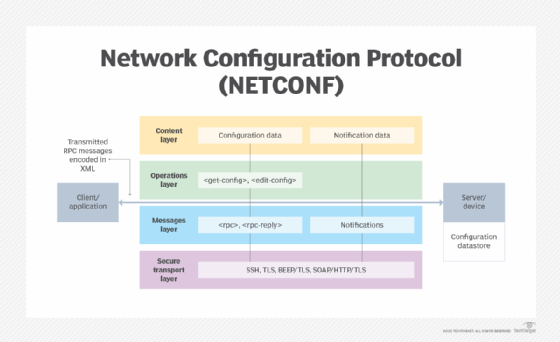
\includegraphics[width=\linewidth]{Images/network_configuration_protocol-f_mobile.png}
    \caption{Diagram illustrating how Network Configuration Protocol (NETCONF) works.}
    \label{fig:example}
\end{figure}

The NETCONF protocol facilitates secure RPC communications between the client and server, providing a standards-based approach to network device management. The protocol can be conceptualized as having four layers:

\begin{itemize}
    \item Secure Transport Layer. The first layer provides the core communication path between the client and server. NETCONF is not bound to any transport protocol, but it can be layered over any transport protocol, including Transport Layer Security and Secure Shell. However, the protocol must provide the necessary functionality. The transport layer makes it possible for the client and server to communicate through a series of RPC messages.
    \item Messages Layer. The second layer provides a transport-independent framing mechanism for encoding RPCs and notifications. NETCONF uses an RPC-based communication model to provide the framing necessary to support requests and responses between the client and server. In documenting the Messages Layer, RFC 6241 focuses primarily on RPC communications, rather than notifications, which are instead documented in RFC 5277.
    \item Operations Layer. The third layer defines a small set of low-level base operations for retrieving information and managing configurations. The set includes operations such as <get-config> or <edit-config>. The operations are invoked as RPC methods with XML-encoded parameters, passed in as child elements of the RPC elements.
    \item Content Layer. The top layer is concerned with configuration and notification data; however, this layer lies outside the scope of RFC 6241. Instead it relies on the device's own data model. NETCONF carries the model's configuration information within the <config> element but treats it as opaque data. The YANG data modeling language (RFC 6020) was developed for specifying NETCONF data models and protocol operations.
\end{itemize}

When a client communicates with a server, it sends one or more RFC request messages to that server, which responds with its own RFC reply messages. The two most common XML elements used for RFC communications are <rpc> and <rpc-reply>. The <RPC> element encloses a request sent from the client to the server. The request information within the element includes the RPC's name and its parameters. The <rpc-reply> element is used to respond to <rpc> messages. All response data is encoded within the <rpc-reply> element.

